% !Mode::"TeX:UTF-8"

% -------------------- Information --------------------

\newcommand{\TITLE}{基于协同过滤和推广格罗夫斯机制的分类匹配推送与竞价机制模型}
\newcommand{\AUTHOR}{}
\newcommand{\SUBJECT}{2019年同济大学数学建模竞赛}
\newcommand{\KEYWORDS}{快速聚类, 协同过滤, 神经网络, 分类匹配推送, 需求显示机制, 格罗夫斯机制}

% -------------------- Packages --------------------

\documentclass[a4paper, 12pt]{ctexart}
\usepackage{amsmath}
\usepackage{amssymb}
% \usepackage{amsthm} % 定理格式 由ntheorem代替.
\usepackage{authblk} % 作者 (见校赛论文).
\usepackage{array}
\usepackage{bigfoot} % to allow verbatim in footnote.
\usepackage{bm} % \bm for bold symbols.
\usepackage{boldline} % 长表格表格线加粗.
\usepackage{caption} % 题注.
\usepackage{commath} % abs, norm
\usepackage{diagbox}
\usepackage{enumerate}
% \usepackage{enumitem} 用enumerate包代替.
\usepackage{filecontents}
\usepackage{flafter} % 不让float出现在定义之前的地方.
\usepackage{float} % 你们这帮float给我乖乖听话 HHHHHHHHHHH.
\usepackage[T1]{fontenc} % Bera Mono Font
\usepackage{fontspec} % 字体.
\usepackage{graphicx}
\usepackage{hyperref}
\usepackage{lastpage}
\usepackage{letltxmacro} % \let
\usepackage{lipsum}
\usepackage{listings} % 排版程序语言.
\usepackage{longtable} % 长表格.
\usepackage{makecell} % 表格线加粗 \Xhline{1.2pt}.
\usepackage{mathtools} % \xleftrightarrow.
\usepackage{mathrsfs} % \mathscr
\usepackage{multirow} % 合并单元格.
\usepackage[square, numbers, sort&compress]{natbib} % 引用.
\usepackage[thmmarks, amsmath, thref]{ntheorem} % 定理格式.
\usepackage[section]{placeins} % 使图像不会显示在别的部分 若过于严格则换成[below].
\usepackage{stackrel} % 上下写 见校赛论文.
\usepackage{subcaption} % subcaption and subfigure
% \usepackage{SUBSubsubsection}
\usepackage{titlesec} % Section标题格式.
\usepackage{varioref} % For Cross References.
\usepackage[dvipsnames]{xcolor} % 颜色声明.
\usepackage{xfrac} %\sfrac{}{}
\usepackage[all, cmtip]{xy} % Commutive diagram.

% Require `xcolor'

\usepackage[numbered, framed]{matlab-prettifier}
\usepackage{pgfplots}
\usepackage{tikz}

% -------------------- Settings --------------------

% Title

\title{\TITLE}
\author{\AUTHOR}
\date{\today}

% Package: caption

\captionsetup{
    margin    =   6pt,
    font      =   small,
    labelfont =   bf
}

% Package: ctex

\setCJKfamilyfont{fzstk}{FZShuTi} % 方正舒体
\newcommand{\fzstk}{\CJKfamily{fzstk}}

% Package: graphicx

\graphicspath{{resources/}} % 图像文件目录

% Package: hyperref

\hypersetup{
    linktoc             =   all,
    colorlinks          =   true,
    linkcolor           =   black,
    anchorcolor         =   black,
    citecolor           =   black,
    filecolor           =   black,
    menucolor           =   black,
    runcolor            =   black,
    urlcolor            =   black,
	pdftitle           	=   {\TITLE},
	pdfauthor          	=   {\AUTHOR},
	pdfsubject         	=   {\SUBJECT},
	pdfcreator			=	{Visual Studio Code},
	pdfproducer			=	{XeLaTeX with documentclass ctexart},
	pdfkeywords        	=   {\KEYWORDS},
    bookmarksnumbered   =   true,
    pdfstartview        =   FitH,
    pdfpagelayout       =   OneColumn
}

% Package: listings

%% Title

\renewcommand\lstlistingname{代码}
\renewcommand\lstlistlistingname{代码}

%% Lstinline with color box

\LetLtxMacro{\oldlstinline}{\lstinline}
\renewcommand{\lstinline}[2][]{\colorbox{lightgray}{\oldlstinline[#1]{#2}}}
\newcommand{\matlabinline}[1]{
    \lstinline[style=MATLAB-editor, basicstyle=\mlttfamily]{#1}}

\lstset{
    breaklines=true,
    backgroundcolor=\color{lightgray},
    basicstyle=\scriptsize,
    inputpath=resources/,
    numbers=left,
    numberstyle={\color{black!33}\scriptsize\sffamily},
    xleftmargin=2em,
    xrightmargin=2em
}

% Package: ntheorem

%% Theorem
\newtheorem{theorem}{Theorem}[section]
\newtheorem{lemma}[theorem]{Lemma}
\newtheorem{corollary}[theorem]{Corollary}
%% Problem
\theoremstyle{plain}
\newtheorem{problem}{Problem}[section]
%% Proposition
\newtheorem{proposition}{Proposition}[section]
%% Conjecture
\newtheorem{conjecture}[proposition]{Conjecture}
%% Definition
\theoremstyle{plain}
\theoremheaderfont{\bfseries}
\theorembodyfont{\rmfamily}
\newtheorem{definition}{Definition}[section]
%% Note
\theoremstyle{plain}
\theoremheaderfont{\itshape}
\theorembodyfont{\itshape}
\newtheorem{note}{Note}[section]
%% Proof
\theoremstyle{nonumberplain}
\theoremheaderfont{\itshape}
\theorembodyfont{\upshape}
\theoremseparator{.}
\theoremsymbol{\ensuremath{\square}}
\newtheorem{proof}{Proof}
%% Solution
\theoremsymbol{\ensuremath{\blacksquare}}
\newtheorem{solution}{Solution}

% Package: pgfplot

\pgfplotsset{width=7cm, compat=1.16}

% Package: varioref

\renewcommand{\reftextbefore}
    {on the \reftextvario{preceding page}{page before}}
\renewcommand{\reftextafter}
    {on the \reftextvario{following}{next} page}
\renewcommand{\reftextfacebefore}
    {on the \reftextvario{facing}{preceding} page}
\renewcommand{\reftextfaceafter}
    {on the \reftextvario{facing}{next} page}
\renewcommand{\reftextfaraway}[1]
    {on page \pageref{#1}}

%% Label formats

\labelformat{lstlisting}{代码#1}
\labelformat{equation}{式(#1)}
\labelformat{figure}{图#1}
\labelformat{table}{表#1}

% -------------------- General new commands --------------------

\DeclareMathAlphabet{\mathsfsl}{OT1}{cmss}{m}{sl}

\DeclareMathOperator{\arcosh}{arcosh}
\DeclareMathOperator{\Arcosh}{Arcosh}
\DeclareMathOperator*{\Beta}{B}
\DeclareMathOperator{\Log}{Log}
\DeclareMathOperator*{\real}{Re}
\DeclareMathOperator*{\image}{Im}

% Expectation

\newcommand{\expect}{\operatorname{E}\expectarg}
\DeclarePairedDelimiterX{\expectarg}[1]{(}{)}{
    \ifnum\currentgrouptype=16 \else\begingroup\fi
    \activatebar#1
    \ifnum\currentgrouptype=16 \else\endgroup\fi
}

\newcommand{\innermid}{\nonscript\;\delimsize\vert\nonscript\;}
\newcommand{\activatebar}{
    \begingroup\lccode`\~=`\|
    \lowercase{\endgroup\let~}\innermid
    \mathcode`|=\string"8000
}

\newcommand*{\BC}{\mathbb{C}}
\newcommand*{\BR}{\mathbb{R}}
\newcommand*{\diff}{\mathop{}\!\mathrm{d}}
\newcommand*{\matr}[1]{\ensuremath{\mathsfsl{#1}}} % italic sans serif
\newcommand*{\me}{\mathrm{e}}
\newcommand*{\mi}{\mathrm{i}}
\newcommand*{\restrict}[1]{\raisebox{-.5ex}{$\vert$}_{#1}}
\newcommand*{\vect}[1]{\bm{#1}}

% -------------------- Specific new commands --------------------



% -------------------- Document --------------------

\begin{document}

    % -------------------- Title Page --------------------

    \maketitle
    \pagestyle{plain}
    \pagenumbering{arabic}

    % -------------------- Abstract Page --------------------

    \newpage
    \begin{abstract}
        % !TeX root = ../main.tex

% 中英文摘要和关键字

\begin{abstract}{代数几何, 交换代数, 准素分解, 维数理论}
  这篇文章主要面向没有接触过但想要了解代数几何的本科生, 旨在以尽可能少的前置知识向读者自洽地展示代数几何的基础.

  代数几何的理论根基在于代数. 本文从基本定义开始建立了以环论为主模论为辅的交换代数理论, 研究了商环与分式环的基本性质, 证明了Noether环上准素分解的存在性及其满足的唯一性, 以域论为基础利用Noether正规化引理证明了域的有限生成整环上的维数定理和Hilbert零点定理.

  代数几何的研究对象在于几何. 本文研究了固定代数闭域上的仿射与射影空间中的代数集, 建立了根式理想与代数集之间的对应, 一次将准素分解理论与几何相联系. 本文还讨论了代数簇上的函数结构, 以此将维数理论应用到几何中, 并证明了两组代数范畴与几何范畴的等价. 最后本文简要介绍了概形的概念, 其相比于代数簇能更完整地体现代数所提供的信息. 读完本文, 读者可以初步掌握代数几何基础, 并做好进一步学习重要技术的准备.
\end{abstract}

\begin{abstract*}{algebraic geometry, commutative algebra, primary decomposition, dimension theory}
  \lipsum[1-2]
\end{abstract*}


        \textbf{关键词:}\KEYWORDS
    \end{abstract}

    % -------------------- Contents --------------------

    \newpage
    \tableofcontents

    % -------------------- Body --------------------

    \newpage

    \section{背景介绍}

    写一本代数几何的入门书籍的困难之处在于如何在提供几何直观和例子的同时推导现代技术的语言. 对于代数几何来说, 作为学科起源的直观想法与现代研究中使用的技术方法有一道巨大的鸿沟.

首当其冲的问题就是语言. 代数几何这门学科经历了很多轮发展, 每一次都有独特的语言和看问题的观点. 十九世纪晚期代数几何有Riemann的函数论方法, 有Brill和Noether的更加几何的方法, 还有Kronecker, Dedekind和Weber的纯代数方法. 同时以Castelnuovo, Enriques和Severi为代表的意大利学派致力于代数曲面的分类. 随后二十世纪以Chow, Weil和Zariski为首的``美国"学派给意大利学派的直观提供了坚实的代数基础. 最近, Serre和Grothendieck创立了法国学派, 他们用概型和上同调的语言重写了代数几何, 并且用心的方法解决了非常多的就问题. 每一个学派都引入了很多新的概念和方法. 在写一本入门书的时候, 是用旧的语言写来贴近几何直观比较好, 还是直接从现代研究中所用的技术语言开始写比较好呢?

第二个问题是一个理念上的问题. 现代数学家倾向于抹去历史的总计: 每一个新的学派都用自己的语言重写这门学科的根基, 这样做有利于严谨性但是不利于教学. 如果一个人知道了概型的定义, 但是却没有意识到一个代数数域的整数环, 一条代数曲线和一个紧黎曼面都是一个``一维正则概型"的例子的话, 那又有什么用呢? 那么这样一本入门书籍的作者应该如何既讲明白代数几何来源于数论, 交换代数和复分析, 又给读者介绍这门学科的主要内容, 即仿射或射影空间上的代数簇, 同时推导概型和上同调这样的现代语言你呢? 有什么样的话题, 可以做到既传达代数几何的意义, 又能作为将来学习和研究的坚实基础呢?

\bigskip

我个人偏向于古典几何这一边. 我相信代数几何中最重要的问题就是那些从老派的仿射空间或射影空间的簇中引出的问题. 他们提供了激发所有后来发展的几何直观. 我以关于簇的一章开始本书, 以最简单的形式建立了一些例子和基本想法, 将它们从技术细节里解放出来. 只有在这些内容都介绍完之后, 我才能系统地建立概型, 凝聚层(coherent sheaves)以及上同调. 这些第二第三章的内容是这本书的技术核心. 在其中我试图陈述一些最重要的结论, 不过不追求一般性. 因此, 比如说上同调理论是针对N\"otherian概型上的拟凝聚层建立的, 因为这比较简单并且对于大多数应用来说已经足够强了; "顺像层(direct image sheaves)的凝聚性(coherence)"定理只证明了射影态射的情况, 并没有对一般的固有态射(proper morphism)进行证明. 因为相同的原因, 我没有引入可表函子(representable functors), 代数空间(algebraic spaces), 平展上同调(\'etale cohomology), sites以及拓扑斯(topoi)这些最抽象的概念.

第四第五章处理了古典的内容, 即非奇异的射影曲线和曲面, 但是运用了概型和上同调的技术. 我希望这些应用可以证明为了发展前两章中的技术所花费的努力是值得的.

关于代数几何的基本语言和逻辑根基, 我才用了交换代数. 它有个好处就是很精确. 并且, 通过在任意特征的域上进行研究, 我们可以获取一些基域是复数域这种古典情形下的洞见. 几年之前, 当Zariski试图编写代数几何的丛书时, 他还需要在书中自己推导需要用到的代数知识. 这项工作占据了全部工作的如此大一部分, 以致于他专门出版了一本只讲交换代数的书. 现在我们十分幸运已经有了很多出色的关于交换代数的书籍. 我关于代数的对策是在需要时引用纯代数的结论, 并给出证明的参考资料. 在书的最后列出了所有用到的代数结论.

原本我计划了完整的一系列附录 - 关于一些当今研究方向的简短介绍, 为了建立这本书的主要内容与研究的桥梁. 因为时间和篇幅有限只有三篇附录得以呈现在成书中. 我十分遗憾这本书中没能包含其余附录, 读者可以去阅读the Arcata volume, 其中有一些针对非专家的由专家所写的关于他们研究领域的文章. 此外, 关于代数几何的历史发展, 可以参考Dieudonn\'e的书. 因为没有足够多的篇幅去像我所希望的那样探索代数几何与相邻领域之间的关系, 可以参考Cassels的关于与数论关系的综述文章, 也可以参考Shafarevich的关于与复流形和拓扑的综述文章.

因为我相信主动学习是一种好的学习方法, 书中有分厂多的习题. 有一些习题包含了正文中没有介绍的重要结论. 其余习题包含了一些能阐释一般理论的具体例子. 我相信对于例子的研究与发展一般理论之间有着不可分割的关系. 认真的学生应该尝试尽可能多地做这些习题, 但是不应该觉得能立即解出他们. 有不少习题需要一些真正有创造性的努力才能够理解. 一个星号表示这道习题是困难的, 两个星号表示这道习题是一个未解决的问题.

(I, \S 8)中有关于代数几何和这本书的进一步介绍.

\subsection*{术语}

大部分情况, 书中的属于与广泛接受的用法是相同的, 不过还是有一些值得注意的例外. \emph{簇}一直是不可约的, 并且一直是在代数闭域上的. 在第一张中所有的簇都是拟仿射的. 在(II, \S 4)中簇的定义被拓展为包括\emph{抽象簇}, 即为代数闭域上的integral separated schemes of finite type, 词语\emph{曲线}, \emph{曲面}和\emph{3-fold}分别用来表示1维, 2维和3维的簇. 但是在第四章中, 词语\emph{曲线}只用来表示非奇异的射影曲线; 在第五章中\emph{曲线}表示任何非奇异射影曲面上的有效除子(effective divisor). 第五章中\emph{曲面}表示非奇异射影曲面.

书中的\emph{概型}在第一版的EGA中被称为预概型(prescheme), 不过在新版EGA中被称为概型.

书中\emph{射影态射}和\emph{very ample invertible sheaf}的定义与EGA中的定义并不等价. 他们在技术上比较简单, 但是有一个缺点就是它并不是基上的局部概念.

词语\emph{非奇异}只对簇使用, 对于一般的概型来说, 我们采用\emph{正则}和\emph{光滑}.

\subsection*{代数的结论}

我假设读者熟悉环, 理想, 模, N\"otherian环, 整相关(integral dependence)的基础知识, 并且乐意接受或者查询其它属于交换代数或者同调代数结论, 这些结论如果需要的话会在书中进行陈述, 伴有相关文本的引用. 这些结论会被标注一个A, 比如说定理3.9A, 为了和书中证明的结论进行区分.

基本的约定有这些: 所有的环都是交换幺环, 单位元记作1. 所有的环同态都将1映到1. 在整环或者域中, $0\neq 1$. 一个\emph{素理想}(或者极大理想)是环$A$的一个理想$\ideal{p}$, 满足商环$A/\ideal{p}$是一个整环(或者域). 因此环本身不被认为是一个素理想或者是极大理想.

环$A$中的一个\emph{乘性系统}(multiplicative system)是一个包含1的子集$S$, 满足关于乘法封闭. \emph{局部化}$S^{-1}A$定义为分式$a/s, a\in A, s\in S$在等价关系下的商, 其中$a/s$与$a'/s'$\emph{等价}仅当存在$s''\in S$使得$s''(s'a-sa')=0$成立. 有两种一直用的局部化列举如下. 设$\ideal{p}$是$A$中的素理想, 那么$S = A - \ideal{p}$是一个乘性系统, 相对应的局部化被记为$A_{\ideal{p}}$. 如果$f$是$A$的元素, 那么$S = \{1\}\cup \{f^n\vert n\geq 1\}$是一个乘性系统, 相对应的局部化被记为$A_f$. (注意在$f$是幂零元的情况下, $A_f$是零环.)

\subsection*{引用}

关于定理, 命题, 引理的交叉引用用圆括号以及数字, 例如(3.5). 对习题的引用例如(习题3.5). 对另一章节的结论的引用以章节数字打头, 例如(II, 3.5)或(II, 习题3.5)


    \section{基于广告和用户分类特征匹配的静态推送模型}

    \subsection{模型假设}

\begin{enumerate}[(1)]
    \item 假设电视台有多个频道,且各频道定位清晰,目标受众有显著差异;
    \item 假设电视台同频道不同时段的节目观众组成大致相同,即同频道不同节目的目标受众分类特征的差异可忽略;
    \item 假设买方对制作的广告定位清晰,且对广告的评估合理;
    \item 假设电视台对其受众的分析精准,能调查了解主要受众的基本信息;
    \item 为简化匹配过程,假设电视频道和视频广告的目标用户分类特征一致.
\end{enumerate}

\subsection{模型建立}

\subsubsection{确定分类特征}

搜集相关资料,我们得知,商业广告在投放时考虑的受众的主要特征如下:

\begin{enumerate}[(1)]
    \item 受众的基本个人信息,如年龄、性别、职业等,这有利于商品精准定位目标受众群体;
    \item 受众的购买力状况,可直接向用户调查了解收入状况,也可通过职业加以判断;
    \item 用户的偏好和收视习惯,可通过获取用户的历史收视和购买记录来获取.
\end{enumerate}

根据假设,电视频道和视频广告的目标用户分类特征一致,
因此再结合以上分析可以考虑将二者的分类特征划分为:

\begin{itemize}
    \item 年龄:依据少年、青年、中年、中老年、老年五个年龄阶段分别以1~5进行表示;
    \item 性别:1代表男性,2代表女性,3代表目标受众无性别上的差异;
    \item 购买力:依据用户的消费能力由低到高由1~5之间的整数表示;
    \item 受教育程度:根据用户的文化程度按小学、初中、普通高中、大专、大专及以上分别以1~5的整数表示;
    \item 消费意愿:根据用户倾向于消费的程度由低到高由1~5之间的整数表示;
    \item 情感倾向:根据用户喜好的情感的表达倾向按理性和感性两级从1~5进行分级.
\end{itemize}

\subsubsection{主成分分析}

以上本文给出了一个将用户分类特征划分为六个属性的示例,
但在实际的分析中模型更为复杂,在数据维数过高的情况下,
一些噪声数据对结果存在较大影响,且模型求解的效率较低.
因此本文为提取变量信息,减少分析的维度,使问题变得更简单、直观,
引入主成分分析的方法来简化模型.其基本步骤如下:

\begin{enumerate}[(1)]
    \item 对所给各项指标进行标准化处理
    \begin{equation}
        Z_{ij}=\frac{x_{ij}-\overline{x_j}}{s_j},(i=1,2,…,n;j=1,2,…,p),
    \end{equation}
    其中,
    \begin{equation}
        \overline{x_j}=\frac{1}{n}\sum\limits_{i=1}^{n}x_{ij},s_j^2=\frac{1}{n-1}
        \sum\limits_{i=1}^{n}(x_{ij}-\overline{x_j})^2(j=1,2,…,p)
    \end{equation}
    \item 根据标准化后的数据矩阵求出相关系数矩阵 $R$
    \begin{equation}
        R=\begin{pmatrix}
        r_{11} & r_{12} & \cdots & r_{1p}\\
        r_{21} & r_{22} & \cdots & r_{2p}\\
        \vdots & \vdots & \ddots & \vdots\\
        r_{n1} & r_{n2} & \cdots & r_{nn}\\
        \end{pmatrix},
    \end{equation}
    其中$r_{ij}(i=1,2,…,n;j=1,2,…,p)$为原变量 $x_i$ 与 $y_j$ 之间的相关系数,其计算公式为
    \begin{equation}
        r_{ij}=\frac{\sum\limits_{k=1}^{n}(x_{ki}-\overline{x_i})(x_{kj}-\overline{x_j})}{\sqrt{\sum\limits_{k=1}^{n}(x_{ki}-\overline{x_i})^2\sum\limits_{k=1}^{n}(x_{kj}-\overline{x_j})^2}}
    \end{equation}
    \item 求出相关系数矩阵 $R$ 的特征根 $\lambda$ 和特征向量 $l$
    \\首先解特征方程$\left| \lambda I-R\right|=0$,可用雅可比法(Jacobi)求出特征值$\lambda_i(i=1,2,\cdots,p)$,并使其按大小顺序排列,$\lambda_1\geq\lambda_2\geq\cdots\geq\lambda_p\geq0$;然后分别求出对应于特征值$\lambda_i$的特征向量$e_i(i=1,2,\cdots,p)$.这里求$\left\|e_i\right\|=1$,即$\sum\limits_{J=1}^{p}e_{ij}^2=1$,其中 $e_{ij}$ 表示向量 $e_i$ 的第 $j$ 个分量.
    \item 计算主成分贡献率及累计贡献率
    \\主成分 $z_i$ 的贡献率:
    \begin{equation}
        \frac{\lambda_i}{\sum\limits_{i=1}^{p}\lambda_i} (i=1,2,\cdots,p)
    \end{equation}
    累计贡献率:
    \begin{equation}
        \frac{\sum\limits_{k=1}^{i}\lambda_i}{\sum\limits_{k=1}^{p}\lambda_i}(i=1,2,\cdots,p)
    \end{equation}
    \item 确定主成分 $F_1,F_2,…,F_k$
    \\一般取累计贡献率达到$85\%-95\%$的特征值 $\lambda_1,\lambda_2,\cdots,\lambda_m$ 所对应的第1,第2,…,第$m(m \leq p)$个主成分 $F_1,F_2,…,F_k$.
\end{enumerate}

\subsubsection{快速聚类($K$均值聚类)}

聚类是研究对样品或指标进行分类的一种多元统计方法,
是一句研究对象的个体的特征进行分类的方法.
聚类分析把分类对象按一定规则分成若干类,这些类非事先给定的,
而是根据某种特征确定的.在同一类中这些对象在某种意义上趋向于彼此相似,
而在不同类中趋向于不相似.

上文中提到了使用主成分分析的方法确定 $p$ 个指标来表示电视频道用户特征,
根据模型假设,本文使用同样的指标来表示视频广告目标用户的用户特征.
接下来,本文通过电视台的频道总数确定一个$K$值,
对买方提供的视频广告进行K均值聚类分析.其基本的过程如下:

\begin{enumerate}[(1)]
    \item 数据无量纲化
    \\由于数据之间的量纲不相同,不便于比较.因此需要对数据进行0-1规格化,即将数据统一放到0~1的范围,将其转化为无量纲的纯数值,便于不同单位或量级的指标能够进行比较和加权.简记特征向量为$A$,则
    \begin{equation}
        v_i'=\frac{v_i-\min(A)}{\max{(A)}-\min{(A)}},v_i\in A    
    \end{equation}
    \item 随机选取 $k$ 个中心点
    \\ 随机选取训练数据中的 $k$ 个点作为起始中心点.
    \item 遍历所有数据,将每个数据划分到最近的中心点中
    \\ 每个样本都有 $p$ 个指标,因此每个样本可以看成 $p$ 维空间中的一个点,可以用距离来度量样本间的接近程度.常用的距离的算法有绝对距离、欧式距离、切比雪夫距离、明考斯基距离.
    \\本文采用欧式距离,即用
    \begin{equation}
        d_{ij}=\sqrt{\sum\limits_{t=1}^{p}(x_{it}-x_{jt})^2}    
    \end{equation}
    来刻画样本 $X_i$ 与 $X_j$ 之间的距离.
\end{enumerate}

\subsubsection{匹配与推送}

上文中,我们得到了广告的 $K$ 个分类,以下简称为广告簇.
可以计算得出各个广告簇的中心向量 $\bm{\alpha_i} (i=1,2,\cdots,k)$,
电视频道用户画像的特征向量 $\bm{\beta_i} (i=1,2,\cdots,k)$
分别计算其两两之间的欧式距离
\begin{equation}
    d=\sqrt{\sum\limits_{t=1}^{p}(\bm\alpha_{it}-\bm\beta_{jt})^2},  
\end{equation}

其中,$i=1,2,\cdots,k;j=1,2,\cdots,k$
将所得结果记录在视频广告簇-电视频道用户(Advertisement-Channel)关联表中,以下简记为广告簇-频道关联表.

然后再根据关联度对广告簇和频道用户进行匹配,其思路如下:

\begin{enumerate}[(1)]
    \item 首先在广告簇-频道表中对应于广告簇的每一行的数据中找到该行的最小欧式距离,
    标记为待定值.
    \item 遍历表中每一行,若该行中的待定值为其所在列(对应于频道)中唯一的待定值,
    则将该值标记为确定值;
    \item 若该行中的待定值不是列中唯一的待定值,则找出这一列中的待定值中的最小值,
    则将该值改为确定值;
    对于该列中其它的待定值所在行,分别在对应未有确定值的列的数据中找到最小欧式距离,
    将该数据标记为确定值;
    \item 重复2,3步,直到表中的每一列和每一行都有且只有一个确定值,该确定值即
    广告簇和频道的一条匹配信息.
\end{enumerate}

最后根据匹配信息,对每个频道推送相应的广告簇

\subsection{模型求解}

针对本模型,本文编纂了以下数据进行求解与验证:

\begin{table}[H]
    \centering
    \caption{电视频道用户分类特征}
    \begin{tabular}{|l|c c c c c c|}
        \Xhline{1.2pt}
        \diagbox{频道}{特征} & 年龄 & 购买力 & 受教育程度 & 情感倾向 & 性别 & 消费意愿 \\
        \Xhline{1.2pt}
        少儿频道 & 1 & 2 & 2 & 5 & 3 & 3 \\
        体育频道 & 2 & 3 & 3 & 5 & 1 & 3 \\
        经济频道 & 3 & 5 & 5 & 1 & 3 & 4 \\
        法治频道 & 4 & 4 & 4 & 2 & 3 & 2 \\
        戏曲频道 & 5 & 1 & 2 & 4 & 2 & 2 \\
        \Xhline{1.2pt}
    \end{tabular}
    \label{tab:my_labe1}
\end{table}

使用SPSS统计分析软件的因子分析功能进行主成分分析,得到的结果如下:

\begin{figure}[H]
    \centering
    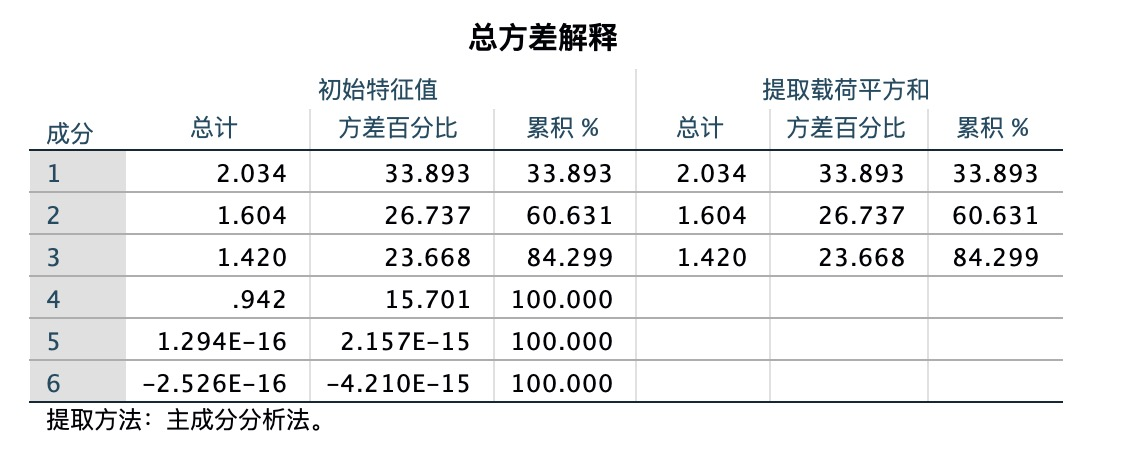
\includegraphics[scale=0.32]{resources/pic1.png}
    \caption{解的总方差}
    \label{pic1}
\end{figure}

根据以上结果,本文应当选取年龄、购买力、受教育程度作为主成分,但考虑到数据量过小导致结果不精确,
本文最终选取了年龄、购买力、受教育程度和情感倾向作为分类特征属性.

接下来,本文编纂了100条按以上述分类特征标记的广告信息,并通过SPSS软件进行快速聚类.聚类的结构如下:

\begin{figure}[H]
    \centering
    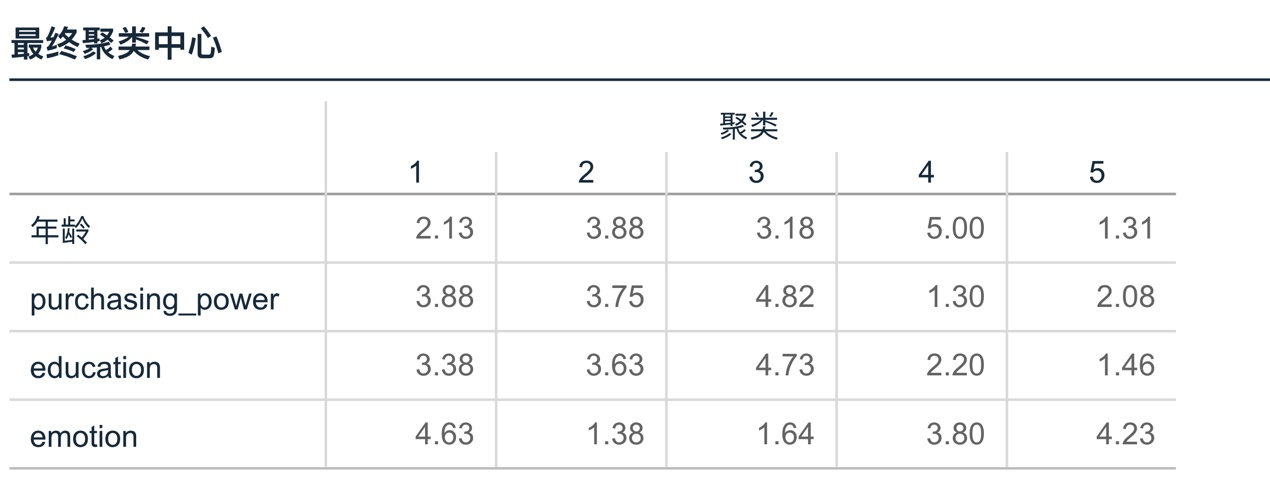
\includegraphics[scale=0.3]
        {resources/pic2.jpg}
    \caption{最终聚类中心}
    \label{pic2}
\end{figure}

对聚类中心和电视频道用户画像特征向量无量纲化并求解欧式距离,可解得:

\begin{table}[H]
    \centering
    \caption{视频广告簇-电视频道用户关联表}
    \begin{tabular}{|l|c c c c c|}
        \Xhline{1.2pt}
        \diagbox{广告簇}{频道} & 少儿频道 & 体育频道 & 经济频道 & 法治频道 & 戏曲频道 \\
        \Xhline{1.2pt}
        广告簇1 & 0.3393 & 0.1363 & 0.5595 & 0.4550 & 0.6157 \\
        广告簇2 & 0.8260 & 0.6206 & 0.2474 & 0.0766 & 0.6374 \\
        广告簇3 & 0.7950 & 0.5921 & 0.0952 & 0.1818 & 0.7631 \\
        广告簇4 & 0.6571 & 0.5481 & 0.7859 & 0.5462 & 0.0608 \\
        广告簇5 & 0.1244 & 0.1870 & 0.8320 & 0.6975 & 0.5964 \\
        \Xhline{1.2pt}
    \end{tabular}
    \label{tab:my_labe2}
\end{table}

根据以上结果,结合上述匹配算法,我们可以得到以下推送关系:

\begin{table}[H]
    \centering
    \caption{推送匹配关系表}
    \begin{tabular}{|c|c|}
        \Xhline{1.2pt}
        \textbf{广告簇} & \textbf{频道} \\
        \Xhline{1.2pt}
        广告簇1 & 体育频道 \\
        广告簇2 & 法治频道 \\
        广告簇3 & 经济频道 \\
        广告簇4 & 戏曲频道 \\
        广告簇5 & 少儿频道 \\
        \Xhline{1.2pt}
    \end{tabular}
    \label{tab:march}
\end{table}

\subsection{模型评价}

本模型的优点有

\begin{itemize}
    \item 本模型实现的方式较为简单,既可以通过编写代码进行匹配和推送,也可使用
    SPSS等统计分析软件对数据进行简单处理后进行匹配;
    \item 本模型实现的时间效率较高,主成分分析和K均值聚类算法均为线性的时间复杂度,
    而最后的匹配算法的时间复杂度为$O(n^2)$,其中 $n$ 为频道数;
\end{itemize}

本模型的缺点有

\begin{itemize}
    \item 本模型需要设定大量的特征分类特征之后,模型的匹配才能更加精确,而分类特征的设定是较耗时的,其拓展性较差;
    \item 本模型的分类特征的取值是人为设定的,存在较大的主观性和臆断性,且容易存在标准尺度不一的情况,对结果有较大影响;
    \item 本模型虽能处理小样本数据,但当广告个数与频道个数的比值过小时,广告特征聚类过于松散,推荐效果较差.
\end{itemize}


    \section{基于市场价和匹配度的保留价估算模型}

    \subsection{模型假设}

出于简化模型的考虑, 本文认为所有的广告视频长度是固定的,
这样就可以把广告总时长的限制转化为广告数量的限制,
可以将拍卖规则设计为前$K$高价者赢得广告播放时段,
其中$K$为该时段能承载的最大广告数量.

假设卖方对广告播放时段的估价为$V_{0}$,
这对买方们来说是公开信息.
记$V_{j}$表示第$j$位买方对广告播放时段的估价.
本文假定本拍卖环境有以下性质:
\begin{enumerate}[({A}1)]
    \item (私有价值) $V_{j}$为各个买方的私人信息,
        对于其余买方而言$V_{j}$为随机变量,
        他们能且仅能知道$V_{j}$的分布, 记累计分布函数为$F_{j}(v_{j})$.
    \item (风险中性) 每个买方的目标是最大化他的期望收益.
    \item (非合作行为) 所有买方之间不存在任何具有约束力的合作性协议.
    \item 以上均为各个买方的公共知识.
\end{enumerate}

\subsection{模型建立}

\subsubsection{估计卖方估价$V_{0}$}

假设广告播放时段的市场价$\tilde{V}_{0}$
与且仅与频道收视率$a_{0}$和频道特征$u_{0}$有关,
那么通过统计回归就可以得出市场价与频道收视率和频道特征的关系,
从而估计某个频道的广告播放时段的市场价.

市场价参数不仅体现了频道收视情况, 也体现了该频道对于广告总体的匹配程度.
比如说少儿频道中受众大多为少年儿童, 与大部分广告内容匹配度低,
因此在收视率相近的情况下,
少儿频道的广告播放时段的市场价会低于卫视广告播放时段的市场价.

因此本文将以市场价$\tilde{V}_{0}$来估计卖方估价$V_{0}$.

\subsubsection{估计买方估价$V_{j}$}

买方估价$V_{j}$取决于他对于播放广告后销售量增加的预期,
而销售量增加的预期取决于收视率以及匹配度. 当卖方固定的时候收视率也固定了,
因此可认为$V_{j}$独立服从于分布$F_{m_{j}}$, 其中参数$m_{j}$为匹配度.

\subsubsection{确定合理保留价}

根据拍卖理论, 如果拍卖机制为第二价格拍卖, 那么每个买方的最优策略即为报出
自己真实愿意付出的价钱$V_{j}$. 赢得广告播放时段之后,
他只需付出报价中低于他报价的最高价即可.

在设计保留价的时候, 卖家需要考虑到保留价过低而造成的广告播放时段以过低价格卖出的风险,
也要考虑到保留价过高而造成的一个广告播放时段中的广告位未能全部卖出的风险.

先考虑一个买方的情况, 简记其私人价值为$V$, 累计分布函数为$F(v)$,
概率密度函数为$f(v)$.
如果卖方定一个保留价$r$, 那么只有在买方的私人价值$V\geq r$
时他才购买其物品, 这一事件发生的概率为$1-F(r)$. 因此, 卖方的期望利润为
\begin{equation}
    \pi(r) = (r-v_{0})(1-F(r)),
\end{equation}
卖方选择最大化$\pi(r)$, 因此最优保留价$r^{*}$满足
\begin{equation}
    r^{*}-\frac{1-F(r^{*})}{f(r^{*})} = v_{0}.
\end{equation}

可以证明如果假设各个买方的私人价值独立同分布,
那么最优保留价仍满足上方程, 并且最优保留价$r^{*}$高于卖方的真实价值$V_{0}$.
本题中各个买方的私人价值不尽相同, 所以本文认为卖方的真实价值$V_{0}$是合理的保留价.


    \section{基于协同过滤和深度学习的动态推送模型}

    \subsection{模型假设}

出于精准针对用户推送的考虑,本文认为买方所能提供的销售记录是个体用户对商品的购买记录,
其中用户的个人的关键信息被隐去,只保留能刻画用户分类特征的一些信息,如性别、年龄和职业信息等。

针对第一题中买方对广告特征的评估存在随意性和主观性的问题,本题中不再需要买方对广告
进行参数化的评价,而只需提供广告类别和广告描述,卖方需要从这两个信息中提炼出广告的特征。

\begin{enumerate}[(1)]
    \item 假设买方在播视频广告的产品都是通过电视广告进行推销的,其它推销方式的影响忽略不计;
    \item 假设买方能准确记录下产品顾客的性别、年龄和职业信息;
    \item 假设买方给电视台提供的销售记录数据服从一定的分布性,能反应其各自受众之间的差异;
    \item 假设买方提供的广告类别准确,且提供的广告描述包含尽量多的关键词信息(包括商品类型、生产商、商品名等)
\end{enumerate}

\subsection{模型建立}

为建立面向已知销售和收视情况的推荐机制,本文提出一种基于深度学习的协同过滤模型。本文使用协同过滤(CollaboratIve Filtering)算法,先计算广告之间的相似度,找到与当前
广告相似的历史广告的销售记录和收看记录,再将这个广告推介给同一用户群体。

协同过滤算法在实际的推荐系统中有着广泛的应用,但在我们的推荐系统中,打分(Rating)矩阵仅由销售和收视情况来决定,则必然会产生打分矩阵稀疏的问题,从而导致推荐效果不理想。
因此,在我们的算法中,加入了深度学习模型和矩阵分解模型,能够从外部辅助信息和传统的打分信息中学习到更为有效地特征表示。

具体的深度学习的模型设计图如下:

\begin{figure}[H]
    \centering
    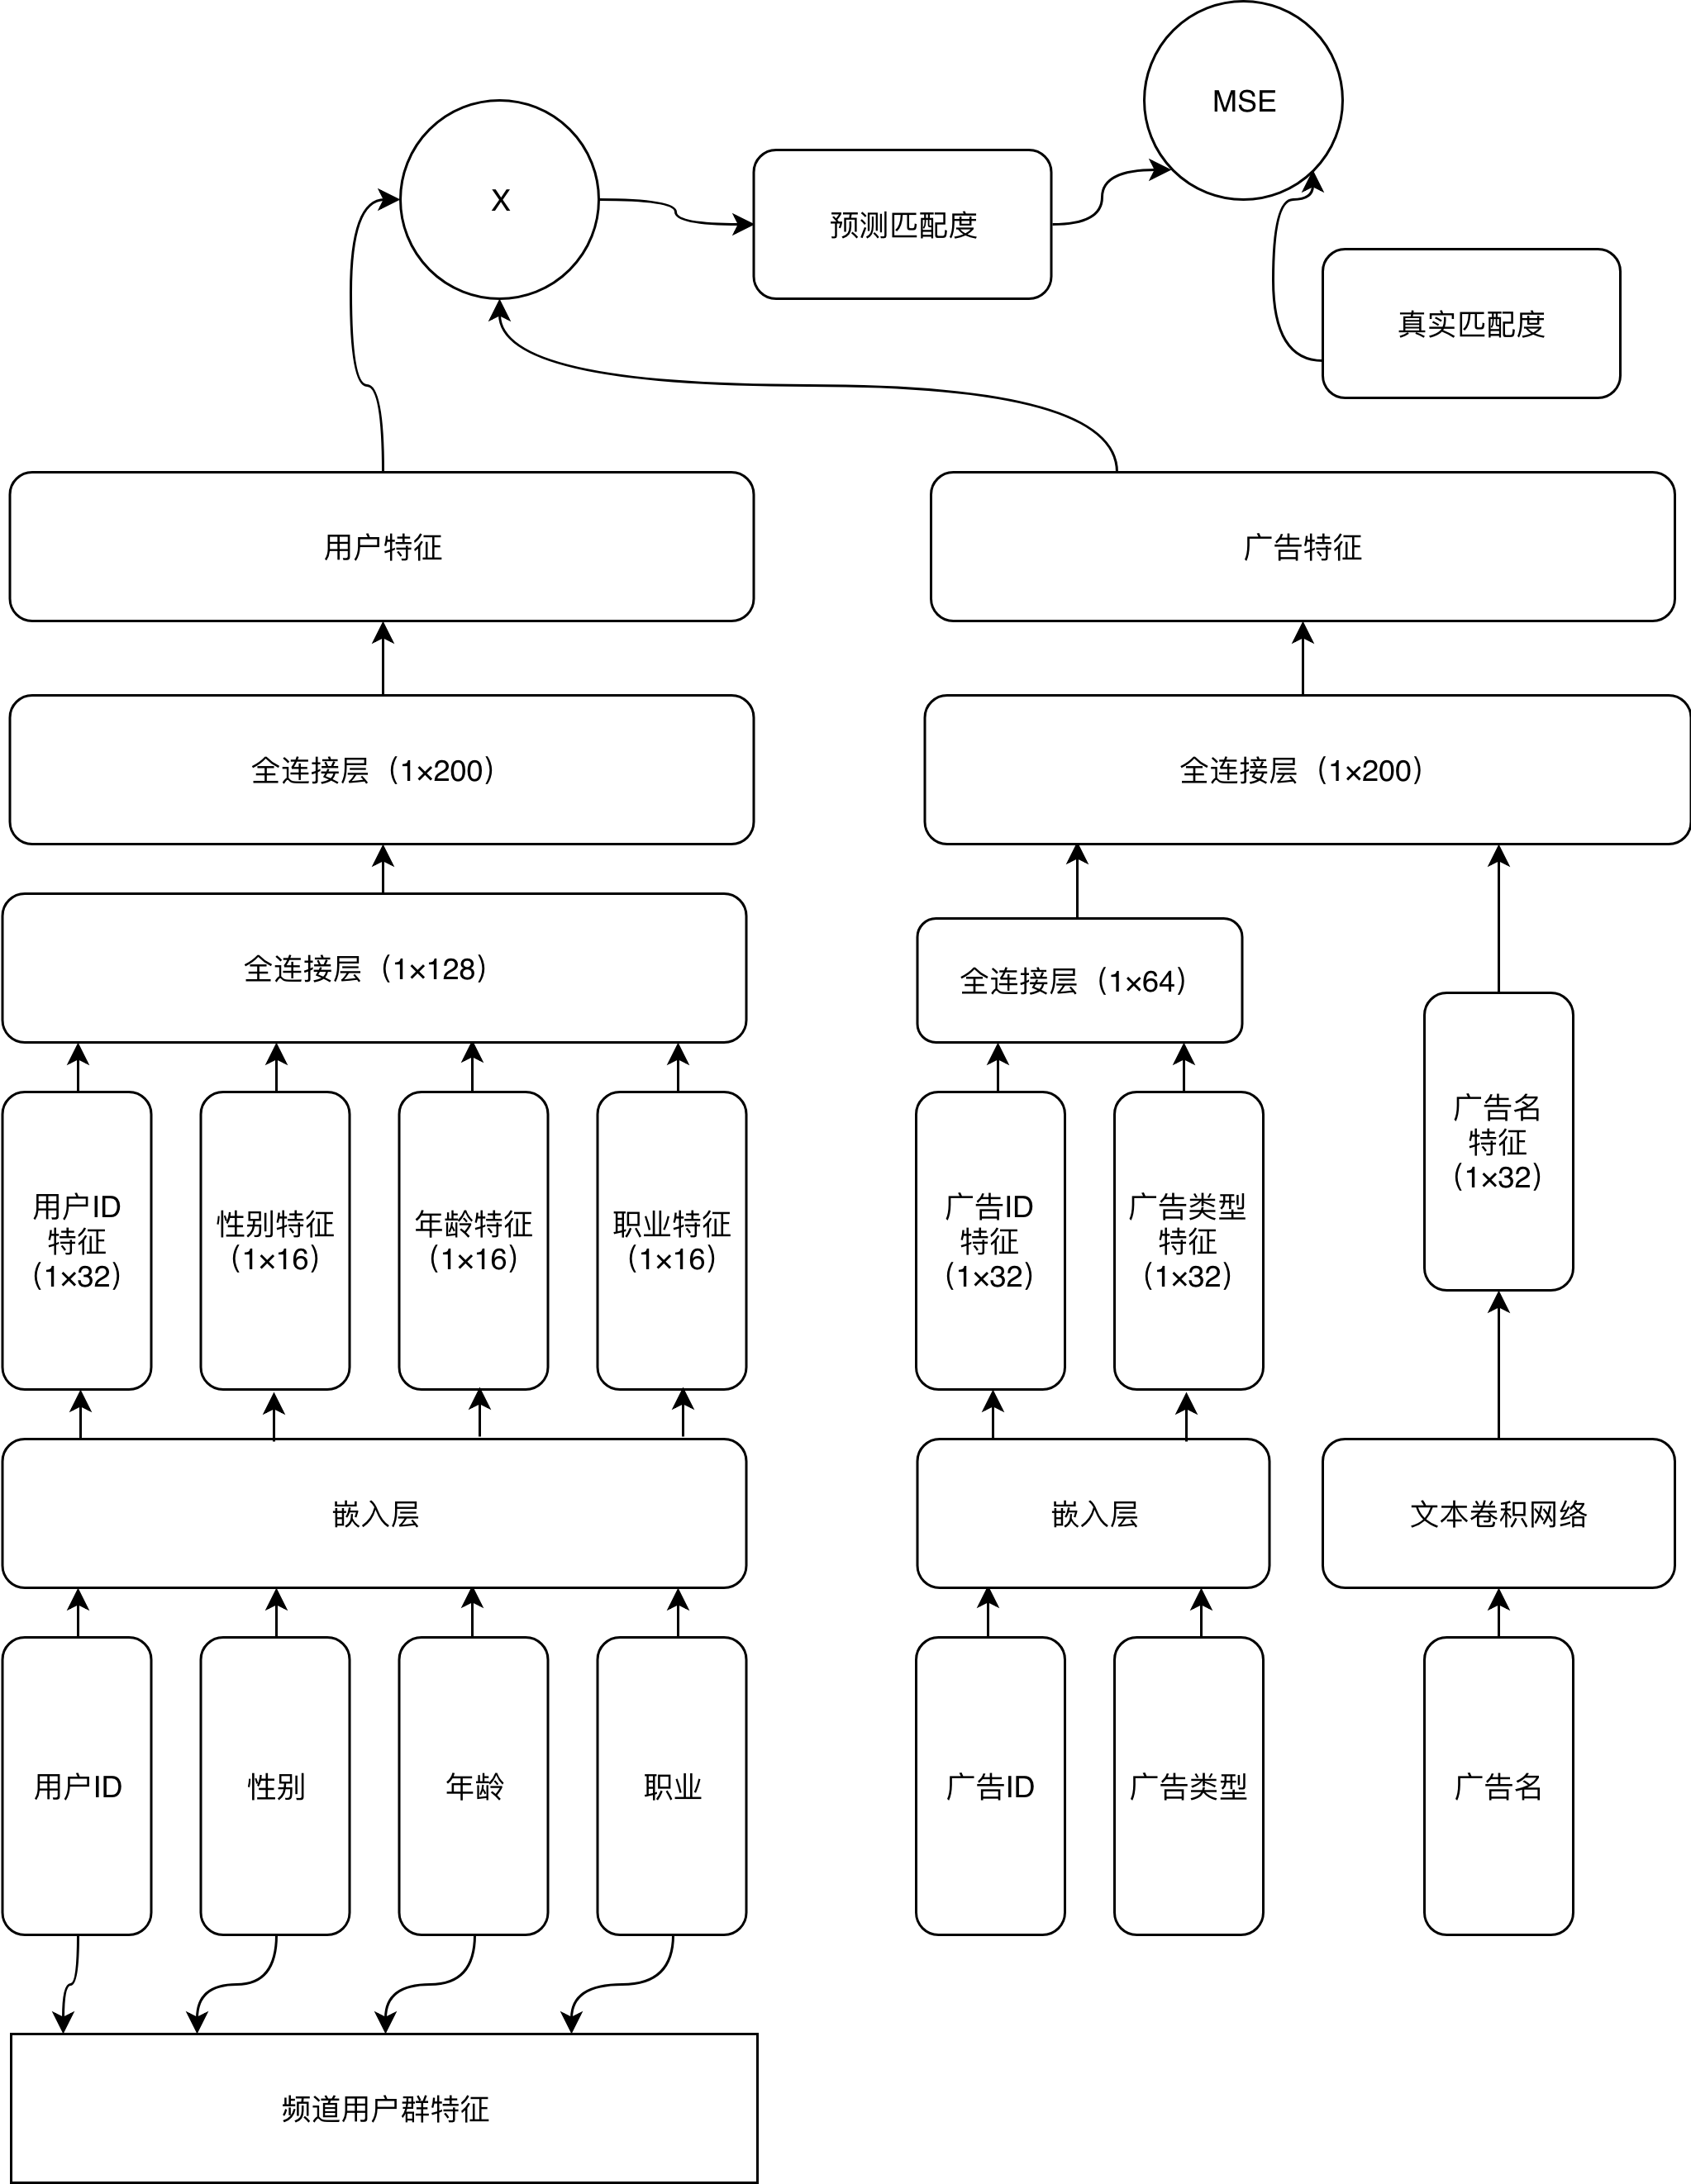
\includegraphics[scale=0.18]
        {resources/Advertisement.png}
    \caption{模型设计}
\end{figure}

\subsubsection{向量化操作}

\begin{enumerate}[(1)]
    \item 首先对数据集进行预处理操作,根据假设,用户数据集中包含了用户的ID、性别、年龄、职业信息,广告数据集中包含了广告类型的信息,为了便于处理,应将这些信息进行数值化处理,其对应关系如下:
    \begin{table}[H]
        \caption{用户年龄性别数值对应表}
        \begin{subtable}[H]{0.5\textwidth}
            \centering
            \caption{用户年龄数值对应表}
            \begin{tabular}{cccc}
            \Xhline{1.2pt}
            0        & 1     & 2     & 3     \\
            \hline
            Under 18 & 18-24 & 25-34 & 35-44 \\
            \Xhline{1.2pt}
            4        & 5     & 6     &       \\
            \hline
            45-49    & 50-55 & 56+   &      \\
            \Xhline{1.2pt}
            \end{tabular}
        \end{subtable}
        \begin{subtable}[H]{0.4\textwidth}
            \centering
            \caption{用户性别数值对应表}
            \begin{tabular}{cc}
            \Xhline{1.2pt}
            0 & 1 \\
            \hline
            女 & 男 \\
            \Xhline{1.2pt}
            \end{tabular}
        \end{subtable}
    \end{table}

    \begin{table}[H]
        \centering
        \caption{用户职业数值对应表}
        \begin{tabular}{cccc}
        \Xhline{1.2pt}
        0                     & 1                   & 2                    & 3                     \\
        \hline
        academic/educator     & artist              & clerical/admin       & college/grad student" \\
        \Xhline{1.2pt}
        4                     & 5                   & 6                    & 7                     \\
        \hline
        customer service      & doctor/health care  & executive/managerial & farmer                \\
        \Xhline{1.2pt}
        8                     & 9                   & 10                   & 11                    \\
        \hline
        homemaker             & K-12 student        & lawyer               & programmer            \\
        \Xhline{1.2pt}
        12                    & 13                  & 14                   & 15                    \\
        \hline
        retired               & sales/marketing     & scientist            & self-employed         \\
        \Xhline{1.2pt}
        16                    & 17                  & 18                   & 19                    \\
        \hline
        technician/engineer   & tradesman/craftsman & unemployed           & writer               \\
        \Xhline{1.2pt}
        \end{tabular}
    \end{table}
    \begin{table}[H]
        \centering
        \caption{广告类型数值对应表}
        \begin{tabular}{ccccc}
        \Xhline{1.2pt}
        0                            & 1                & 2                  & 3              & 4             \\
        \hline
        Life-style                   & Advertising-song & Purchase-reason    & Intuitive      & Visual-effect \\
        \Xhline{1.2pt}
        5                            & 6                & 7                  & 8              & 9             \\
        \hline
        Emotional                    & Humor            & Customer-recommend & Story          & Pleasant      \\
        \Xhline{1.2pt}
        10                           & 11               & 12                 & 13             & 14            \\
        \hline
        Passionate                   & Cartoon          & Rational           & Leben-passiert & Persuasive    \\
        \Xhline{1.2pt}
        15                           & 16               & 17                 & 18             &               \\
        \hline
        \textless{}PAD\textgreater{} & Demonstration    & Single-speaker     & Film           &              \\
        \Xhline{1.2pt}
        \end{tabular}
    \end{table}
    \item 接着用这些数字当做嵌入矩阵的索引,在网络的第一层使用了嵌入层,其维度是($N$,32)和($N$,16);
    \item 针对广告描述这段文本内容,本文采用了文本卷积网络的方式进行处理。
    先由每一个单词的嵌入向量组成的嵌入矩阵,然后接下来下一层使用多个不同尺寸(窗口大小)
    的卷积核在嵌入矩阵上做卷积,窗口大小指的是每次卷积覆盖几个单词。最后得到一个长向量,
    使用dropout做正则化,最终得到广告描述的向量;
    \item 从嵌入层索引出特征以后,将各特征传入全连接层,将输出再次传入全连接层,最终分别得到(1,200)的用户特征和广告特征两个特征向量。
\end{enumerate}

\subsubsection{训练网络}

本文在训练网络层次参考借鉴了Collective Matrix Factorization模型\citep{Singh}。

\begin{figure}[H]
    \centering
    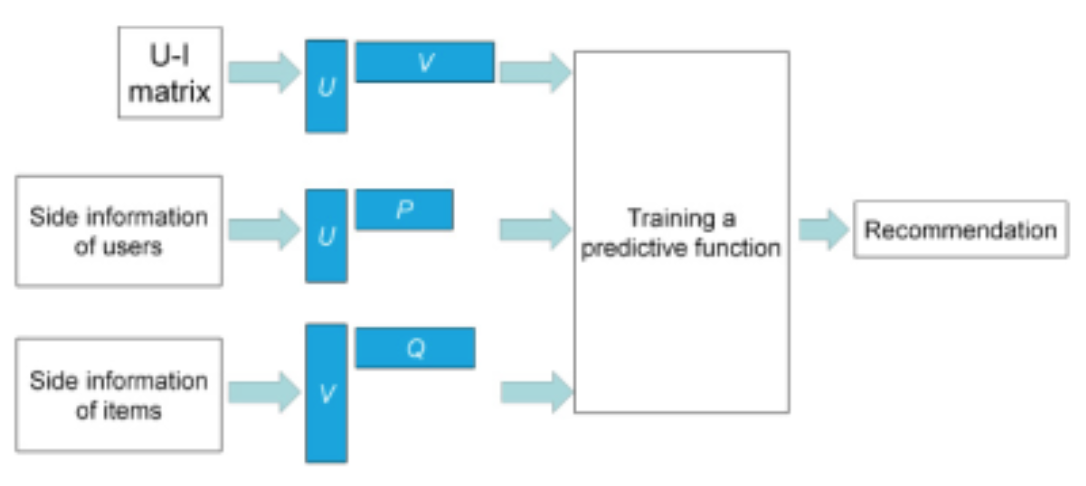
\includegraphics[scale=0.75]{cmf.png}
    \caption{Collective Matrix Factorization}
\end{figure}

这里CMF模型通过分别分解打分矩阵$\matr{R}$,用户、广告的辅助信息矩阵,
其中用户和广告出现在多个矩阵中,其所分解的隐向量都是一致的、共享的,从而建立联系。

在上述深度学习的模型的具体实现中,本文使用了激活函数ReLu来实现模型的优化:
\begin{equation}
    f(x)=\max(0,x)
\end{equation}

\begin{figure}[H]
    \centering
    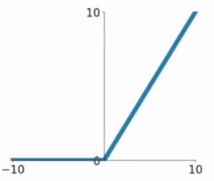
\includegraphics[scale=0.8]{ReLu.png}
    \caption{ReLu激活函数}
\end{figure}

其对于模型的优化在于:
\begin{itemize}
    \item 在输入为正数的时候,不存在梯度饱和问题;
    \item 计算速度有较大提升。ReLU函数只有线性关系,因此不管是前向传播还是反向传播,
    都会比sigmod函数和tanh函数要快很多。因为sigmod函数和tanh函数都需要计算指数,
    所以计算速度会比较慢。
\end{itemize}
当然,经过测试,我们也发现了一些缺点:
\begin{itemize}
    \item 当输入是负数的时候,ReLU是完全不被激活的,这就表明一旦输入到了负数,
    ReLU就会失效。这样在前向传播过程中,问题还没有显露,有的区域是敏感的,
    有的是不敏感的。但是到了反向传播过程中,输入负数,梯度就会完全降到0,
    这个和sigmod函数、tanh函数有一样的问题。
    \item ReLU函数的输出要么是0,要么是正数,这也就是说,
    ReLU函数不是以0为中心的函数。
\end{itemize}

\subsubsection{预测与推荐}

在协同过滤算法中,将特定的广告推送给用户的实质就是预测用户对该广告的评分,并将
对其评分最高的$N$个用户作为推送的对象。

\begin{itemize}
    \item 给定打分矩阵$ \matr{R}\in \BR^{m\times n}$,用户和广告的辅助信息分别是
    $ X\in \BR^{m\times p}$ 和 $Y\in \BR^{n\times q}$;
    \item $u_i,v_j \in \BR^{k}$ 分别表示分别表示第$i$个用户和第$j$个广告的隐含特征向量,
    k 表示维度,那么$ U=u_{1:m},V=v_{i:n}$ 就是我们学习的目标———用户和广告的隐含表示,
    进而预测用户对广告的打分;
    \item 从矩阵分解的角度来说,就是求解
    \begin{equation}
        \arg \min_{U,V} \mathcal{L}(R,UV^{\top})+\lambda(\abs{U}_F^2+\abs{V}_F^2)
    \end{equation}
    的过程。
\end{itemize}

在这里本文将基于用户的协同过滤算法与基于广告的协同过滤算法相结合,在上面方法实现的基础上寻求另一种求解的可能。

假设需要预测用户$A$对广告$M$的评分,首先对于广告$M$,根据训练数据集找出通过广告$M$购买商品的用户,
然后计算$A$和这些用户之间的相似度,依据相似度和这些用户对$M$的购买倾向,来预测用户$A$对广告$M$的评分。

在模型求解的过程中,我们发现根据训练数据集找出已经通过该电视广告购买商品的用户较容易,
预测结果的优劣关键在于如何计算用户$A$和这些
用户之间的相似度,以及采用何种方式来利用相似度和评分预测出用户$A$对广告$M$的购买倾向。其具体计算过程如下:

\begin{itemize}
    \item 首先,对于待预测的用户-广告(User::Advertisement)对,找出对于该广告已有购买记录的用户群Users[s];
    \item 然后,计算该用户与这些用户的余弦相似度$sim(u,i)$
    \begin{equation}
        sim(u,i)=\cos\theta=\frac{\sum\limits_{t=1}^{n}(u_t\times a_t)}{\sqrt{\sum\limits_{t=1}^{n}u_t^2}\times \sqrt{\sum\limits_{t=1}^{n}a_t^2}}
    \end{equation}
    \item 最后,利用
    \begin{equation}
        prescore(u,m)=\frac{\sum\limits_{i\in Users[s]}(sim(u,i)\times score(i,m))}{\sum\limits_{i\in Users[s]}sim(u,i)}
    \end{equation}
    预测用户$u$对广告$m$的购买倾向。
\end{itemize}

\subsection{模型求解}

由于本模型的求解需要大量的数据,而我们难以在互联网中找到类似的资源,因此本文
采用了推荐算法常用的开源数据集MovieLens数据集。
该数据集包含多个用户对多部电影的评级数据,也包括电影元数据信息和用户属性信息。
本文在引入该数据集时对该数据集做了一定的改动:
\begin{enumerate}
    \item 删除了一些不需要用户和物品的信息;
    \item 将原数据集中的电影名属性替换成了广告描述。
\end{enumerate}

本文的验证过程在Jupyter Notebook环境下。受制于正文篇幅限制,本文将代码和运行结果放在附录中。
此处只展示训练模型的均方差(MSE)结果:

\begin{figure}[H]
    \centering
    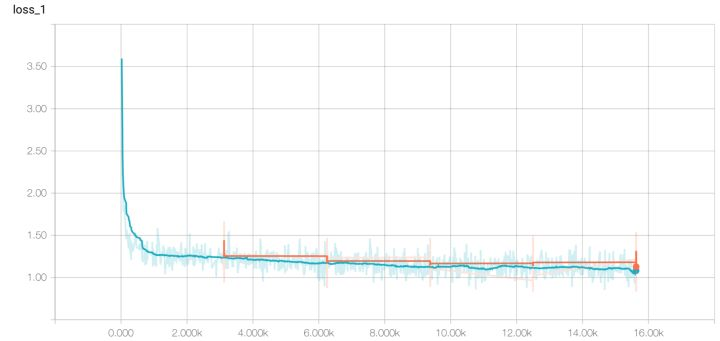
\includegraphics[scale=0.5]{TensorBoard.jpg}
    \caption{TensorBoard可视化结果}
\end{figure}

\subsection{模型评价}

经分析,本模型的优点如下:
\begin{itemize}
    \item 融合了外部辅助信息,学习的用户、广告表示较为丰满;
    \item 融合了历史数据,可以实时更新模型,从而动态地产生推荐;
    \item 虽模型训练时间花费较大,但模型训练后产生推荐相应速度很快。
\end{itemize}

本模型的缺点有:

\begin{itemize}
    \item 本模型采用的CMF方法中,特征的融合方式是直接将各向量首尾相连,这种融合过于简单直白,学习到的用户和广告的隐藏向量表示存在缺陷。
\end{itemize}


    \section{基于需求显示机制和动态匹配度的竞价机制模型}

    \subsection{模型假设}

与前题相同, 假设广告视频长度固定, 并且额外假设当频道和时段固定时,
广告播放对买方带来的收益分布与广告与频道的动态匹配度呈正相关,
而与被广告物本身的价值无关.

\subsection{模型建立}

在本题中需要建立竞价交易模型,
极大化卖方收益的同时提升收视率和买方产品销售量.

本文按如下方式建立经济模型: 固定频道特征和广告播放时段,
设共有$n$个买方为潜在的参与竞价者,
他们可以有放弃竞价的权利.
买方$i$的经济特征$e_{i}$即为买方广告的动态匹配度$a_{i}$和买方的报价$b_{i}$.
记社会选择函数$f$为从经济环境$E$到可行配置结果空间$Y$的映射,
其中可行配置结果空间$Y$包含赢得竞价的买家和其应付的价格$p_{i}$.
应满足动态匹配度$a_{i}$和报价$v_{i}$都尽可能高.
本文寻找的经济机制需要使得对所有的经济环境$e\in E$都有其配置结果符合社会选择.

经济机制在竞价之前公开给所有买方, 它由信息空间$M$和配置规则函数$h$所组成,
其中信息空间内的元素$m$包含买方的报价以及买方广告的动态匹配度,
而配置规则函数$h$根据信息$m$决定赢得竞价的买方.

在本题中, 对于配置结果$y\in Y$, 如果买方$i$赢得竞价, 即$i\in y$,
那么买方所获得的效益为他的真实估价$v_{i}$减去付出的价格$p_{i}(y)$,
其中真实估价$v_{i}$与配置结果$y$无关;
如果买方$i$未赢得竞价, 则效益为0, 即买方$i$的价值函数可写为
\begin{equation}
    u_{i}(y) = \chi_{y}(i)(v_{i}-p_{i}(y)).
\end{equation}
设卖方对于把广告播放时段卖给动态匹配度为$a_{i}$的买家$i$的估价为$F_{i}=F(a_{i})$,
记$\Delta F_{i}=F_{i} - F$, 其中$F$为平均估价,
那么卖方的价值函数可写为
\begin{equation}
    u(y) = \sum_{i=1}^{n}{\chi_{y}(i)(p_{i}(y)-F_{i})}.
\end{equation}

直观上本题中设立的经济机制需要能够诱导买方报出他们的真实估价$v_{i}$,
如此一来根据假设, 动态匹配度高的买方愿意出较高的价格赢得竞价.
由于买方的报价接近于他们对广告播放时段的估价, 并不会恶意拉低报价,
所以卖方的收益得以保证; 与此同时由于动态匹配度高的广告得到播放,
那么电视观众较愿意观看广告也较愿意购买产品, 于是收视率不会被拉低,
买方产品销售量也能提升.

于是文献\citep{Tian}中提到的格罗夫斯-克拉克-威克瑞(Groves-Clark-Vickrey)
需求显示机制能很好地解决本题中涉及到的问题.
本文推广了原始的格罗夫斯机制, 引入了动态匹配度对于卖方估价的影响,
从而引入了动态匹配度对买方报价的修正.
以下我们先假定有且仅有一个买家能赢得广告播放时段.

首先格罗夫斯机制要求每个买方$i$报出他的报价$b_{i}$. 每个人的报价有真有假,
因此$b_{i}$不一定等于$v_{i}$. 然后根据报价与卖方估价的差$b_{i}-F_{i}$是否为最大值
决定买方是否赢得竞价, 即格罗夫斯机制规定赢得竞价的买方由下式决定
\begin{equation}
    y(b) = i, \quad \text{if}\ b_{i}-F_{i} = \max_{j}{(b_{j}-F_{j})}.
\end{equation}

每个买方$i$的转移支付(transfer payment)记为$t_{i}$,
若$t_{i}<0$则被解释为附加税, 若$t_{i}>0$则被解释为补偿.
$t_{i}$体现了买方$i$的报价对于其余买方收益的影响, 由下式决定
\begin{equation}
    t_{i}(b) =
    \begin{cases}
        \displaystyle\sum_{j\neq i}b_{j} + d_{i}(b_{-i}),
        &\text{if}\ b_{i}-F_{i} = \displaystyle\max_{j}{(b_{j}-F_{j})},\\
        d_{i}(b_{-i}), &\text{else}.
    \end{cases}
\end{equation}
这里$d_{i}$是可任意给定的函数. 于是买家$i$的支付函数为
\begin{equation}
    p_{i}(y(b))=
    \begin{cases}
        v_{i}+\displaystyle\sum_{j\neq i}b_{j} + d_{i}(b_{-i}),
        &\text{if}\ b_{i}-F_{i} = \displaystyle\max_{j}{(b_{j}-F_{j})},\\
        d_{i}(b_{-i}), &\text{else}.
    \end{cases}
\end{equation}

可以证明每个人真实显示他的估价$v_{i}$是优势均衡策略, 即每个人都有激励说真话.
由于$d_{i}$为任意给定函数, 所以我们不妨令
\begin{equation}
    d_{i}(b_{-i}) = -\max_{y}{\sum_{j\neq i}{b_{i}(y)-\Delta F_{i}(y)}},
\end{equation}
则转移支付函数变为
\begin{equation}
    t_{i}(b)=\sum_{j\neq i}{b_{j}} - \max_{y}{\sum_{j\neq i}{b_{i}(y)
    -\Delta F_{i}(y)}}.
\end{equation}
在本竞价机制中, 如果$i$赢得竞价, 则$\sum_{j\neq i}{b_{j}}=0$, 于是
$t_{i}(v)=-\max_{j\neq i}{b_{j}}$. 如果$i$未赢得竞价,
则$t_{i}(v)=0$. 所以$b_{i}-\Delta F_{i}$最高的买方赢得竞价,
而最终出价为第二高未修正报价.

上文的讨论是基于只有一个买家能赢得广告播放时段进行的,
事实上可以直接推广到有限个买家能赢得广告播放时段的情形.
设共有$K$个赢家, 先将多赢家竞价问题分解为$K$个单赢家竞价问题:
每个买方在每次竞价中的出价独立, 每次竞价取修正出价最高的买方赢得广告播放时段,
实际出价为第二高价, 赢得广告播放时段的买家不参与下一次竞价.
而事实上之前已经证明了在单赢家竞价模型中买方报出真实估价为优势均衡策略,
因此可以假设每个买方在各次竞价中出价相同, 所以多赢家竞价机制即为:
修正报价前$K$高的买方赢得广告播放时段, 实际出价为排名比他低一位的未修正报价.

至此本文得到了基于动态匹配度的推广格罗夫斯竞价交易机制,
它能较好地解决电视台广告竞价问题.


    \section{结论}

    针对问题一, 本文设计了一个基于快速聚类算法的静态推荐模型,
实现了推送给电视频道与其相似度高的广告.

针对问题二, 本文通过分析设置保留价对竞价带来的变化, 退出保留价应与卖方估价相近,
从而得到合理保留价.

针对问题三, 本文设计了一个基于协同过滤和深度学习的动态推荐模型,
比传统算法能更有效地去刻画广告和用户的特征.

针对问题四, 本文从经济机制理论出发, 推广了格罗夫斯机制,
结合本问题的经济环境得到了具体的经济机制.


    % -------------------- Bibliography --------------------

    \newpage
    \bibliography{bibliography}
    \bibliographystyle{plain}

    % -------------------- Appendix --------------------

    \newpage
    \appendix

    \section{广告推荐协同过滤算法的代码}

    \lstinputlisting[
        caption=广告推荐协同过滤算法,
        basicstyle=\mlttfamily\scriptsize
        ]{Advertisement_Recommend.md}

\end{document}
